\documentclass[11pt]{article}

%------------------------------------------------
% Packages and formatting
%------------------------------------------------
\usepackage[margin=0.8in]{geometry}
\usepackage[utf8]{inputenc}
\usepackage[T1]{fontenc}
\usepackage{setspace}
\usepackage{amsmath, amssymb}
\usepackage{graphicx}
\usepackage{xcolor}
\usepackage{hyperref}
\usepackage{booktabs}
\usepackage{tikz}
\usetikzlibrary{arrows.meta, positioning, shapes.geometric, calc}

\onehalfspacing

%------------------------------------------------
% Listings setup for code/terminal
%------------------------------------------------
\usepackage{listings}

\definecolor{codebg}{RGB}{248,248,248}
\definecolor{codeframe}{RGB}{220,220,220}
\definecolor{bashkw}{RGB}{0,0,150}
\definecolor{pykw}{RGB}{120,0,120}
\definecolor{codestring}{RGB}{0,120,0}
\definecolor{codecomment}{RGB}{120,120,120}

\lstdefinestyle{bashstyle}{
  language=bash,
  basicstyle=\ttfamily\scriptsize,
  keywordstyle=\color{bashkw}\bfseries,
  stringstyle=\color{codestring},
  commentstyle=\color{codecomment}\itshape,
  showstringspaces=false,
  columns=fullflexible,
  frame=single,
  framerule=0.4pt,
  rulecolor=\color{codeframe},
  backgroundcolor=\color{codebg},
  breaklines=true,
  breakatwhitespace=true,
  keepspaces=true
}

\lstdefinestyle{pythonstyle}{
  language=Python,
  basicstyle=\ttfamily\scriptsize,
  keywordstyle=\color{pykw}\bfseries,
  stringstyle=\color{codestring},
  commentstyle=\color{codecomment}\itshape,
  showstringspaces=false,
  columns=fullflexible,
  frame=single,
  framerule=0.4pt,
  rulecolor=\color{codeframe},
  backgroundcolor=\color{codebg},
  breaklines=true,
  breakatwhitespace=true,
  keepspaces=true
}

\lstset{escapeinside={(*@}{@*)}}

%------------------------------------------------
% Title
%------------------------------------------------
\title{Workflow for Preparing DHSVM Input Files \\ Using QGIS--GRASS and a Pure Python Pipeline\\
\large (AR Watershed Example)}
\author{Yiyun Song}
\date{\today}

\begin{document}
\maketitle

\section{Overview}

This document describes an end-to-end, pure Python workflow for preparing all required spatial and state input files for DHSVM for the AR watershed. The updated pipeline replaces legacy intermediate ASCII exports and C-engine utilities with direct binary serialization. It combines:

\begin{itemize}
  \item QGIS with GRASS GIS for fundamental spatial preprocessing (DEM clipping, flow accumulation, stream extraction).
  \item A unified Python master script (\texttt{prep\_dhsvm\_inputs.py}) that coordinates topological routing, binary grid generation, and physical initial state computation.
\end{itemize}

All paths in this document use the example project directory:
\begin{quote}
\texttt{/Users/benthosyy/Desktop/CreateStreamNetwork\_PythonV/DEM\_AR\_0406}
\end{quote}

\section{Directory Structure and Prerequisites}

The workflow enforces strict directory routing to separate intermediate diagnostic artifacts from production-ready model inputs. This keeps the workspace organized and prevents accidental file overwrites during calibration.

\paragraph{Source directories (user-maintained):}
\begin{itemize}
  \item \texttt{Reprojected\_DEM/} -- Reprojected master DEMs.
  \item \texttt{Reprojected\_Watersheds/} -- Watershed polygon(s) in the working CRS.
  \item \texttt{scripts/} -- Custom Python modules (detailed in Section~\ref{sec:modules}):
        \begin{itemize}
          \item \texttt{prep\_dhsvm\_inputs.py} (Master orchestrator)
          \item \texttt{rowcolmap.py}, \texttt{roadaspect.py} (Row/Col indexing \& stream aspect)
          \item \texttt{channelclass.py} (Channel classification)
          \item \texttt{soildepthscript.py} (Topographic soil depth)
          \item \texttt{dem\_to\_dhsvm\_bins.py} (Base map serialization)
          \item \texttt{generate\_dhsvm\_states.py} (Initial state generator)
          \item \texttt{plot\_mainstem.py} (Geomorphic validation)
        \end{itemize}
\end{itemize}

\paragraph{Automatically generated output directories:}
\begin{itemize}
  \item \texttt{DHSVM\_input\_binaries/} -- Flat binary grids (DEM, mask, soil, veg, depths).
  \item \texttt{DHSVM\_input\_streams/} -- Topological files (map, network, class).
  \item \texttt{modelstate/} -- Pure Python generated initial condition grids and channel states.
  \item \texttt{Intermediate\_GIS/} -- Diagnostic rasters and shapefiles for QA.
\end{itemize}

\section{Pipeline Architecture and Module Functionality}
\label{sec:modules}

The pipeline uses a modular Python architecture. Each script addresses a specific physical or computational requirement of DHSVM, so that individual stages can be modified or swapped without destabilizing the rest of the workflow.

\subsection{Core Python Modules}
\begin{itemize}
  \item \textbf{\texttt{prep\_dhsvm\_inputs.py}} (Master Script): Orchestrates the entire workflow within the QGIS environment. It sequences the GRASS processing and dynamically imports all sub-modules through \texttt{importlib}, allowing each stage to be updated independently.
  \item \textbf{\texttt{rowcolmap.py} \& \texttt{roadaspect.py}}: Essential geometric utilities. They map geographic coordinates to DHSVM's row/column matrix indices (with a top-left origin consistent with DHSVM map files) and compute local stream aspect to align surface runoff partitioning. \texttt{rowcolmap.py} also assigns deterministic \texttt{SegID} values to stream segments and performs a uniqueness sanity check.
  \item \textbf{\texttt{channelclass.py}}: Classifies vector stream segments based on topographic slope and upstream contributing area, generating the structured \texttt{stream.class.dat} routing table. Slope units (degrees, percent, or tan) are auto-detected from the attribute distribution and internally converted to $\tan(\theta)$ before binning, which makes the module portable across different GRASS output conventions.
  \item \textbf{\texttt{soildepthscript.py}}: Replaces constant depth assumptions by generating a topographically weighted soil depth raster using the PNNL weighted formula (slope, source area, and elevation terms). Parameters are calibrated to the Southern Appalachians / Coweeta Hydrologic Laboratory regime (\texttt{MIN\_DEPTH}~=~2.0\,m, \texttt{MAX\_DEPTH}~=~6.0\,m). It enforces the DEM mask as an absolute master mask so that boundary pixels lost by upstream 3$\times$3 raster operations are restored, guaranteeing perfect pixel alignment for the DHSVM C-engine.
  \item \textbf{\texttt{dem\_to\_dhsvm\_bins.py}}: Reads the foundational DEM and writes DHSVM-ready Float32 and Int8 base map binaries (\texttt{dem.bin}, \texttt{mask.bin}, \texttt{soil.bin}, \texttt{veg.bin}) directly via NumPy. It simultaneously generates a suite of uniform soil depth baselines (2.0\,m through 4.0\,m) that share the exact same spatial mask as the dynamic depth raster, enabling strictly pixel-aligned sensitivity experiments.
  \item \textbf{\texttt{generate\_dhsvm\_states.py}}: Initializes the cold-start conditions for the model. It writes Float32 grid states directly as flat binaries (with \texttt{.bin} explicitly appended to satisfy DHSVM's internal \texttt{ReadModelState} path concatenation), and dynamically parses \texttt{stream.class.dat} to compute physically accurate initial water volumes for each channel segment ($V = W \cdot L \cdot d_0$).
  \item \textbf{\texttt{plot\_mainstem.py}} (Validation): A standalone analytical tool that traces the true physical main stem upstream from the outlet by enforcing elevation-based routing on the extracted stream network. It identifies geomorphic knickpoints via smoothed slope thresholds and exports longitudinal profile data and figures for quality assurance.
\end{itemize}

\subsection{Rationale for a Pure Python Architecture}

The transition from legacy methods (ASCII exports, \texttt{myconvert}, \texttt{MakeModelStateBin}, \texttt{MakeChannelState.sh}) to a pure Python pipeline resolves several long-standing computational and physical inconsistencies:

\begin{enumerate}
    \item \textbf{Direct Binary Serialization:} NumPy's \texttt{tofile()} translates raster arrays directly into memory-contiguous Float32 and Int8 binaries. This eliminates the floating-point precision truncation inherent in ASCII text conversion, bypasses the OS-dependent \texttt{myconvert} utility, and reduces I/O execution time by roughly an order of magnitude.
    \item \textbf{Dynamic Channel Width Parsing:} The legacy bash script (\texttt{MakeChannelState.sh}) hardcoded channel widths for a limited number of stream classes. For higher-order classes (e.g., Class~13), this resulted in unassigned widths, yielding initial channel volumes of zero and subsequent numerical shocks during the model spin-up phase. \texttt{generate\_dhsvm\_states.py} resolves this by dynamically parsing \texttt{stream.class.dat}, guaranteeing physical conservation of mass for any classification scheme.
    \item \textbf{Circumventing C-Engine Memory Limitations:} Legacy utilities like \texttt{MakeModelStateBin} possess a hardcoded \texttt{NAMESIZE} buffer limit (typically 128 characters). Deeply nested project directories cause path concatenations to exceed this limit, triggering buffer overflows (Segmentation Faults / \texttt{SIGFPE} / trace traps). By writing the binary arrays natively in Python and explicitly appending the \texttt{.bin} extension, the pipeline conforms to DHSVM's \texttt{ReadModelState} I/O requirements without invoking the vulnerable C memory constraints.
    \item \textbf{Endianness Compatibility:} The Python pipeline natively generates little-endian binaries that are bit-for-bit compatible with the DHSVM \texttt{ReadModelState} C-routines on the target platforms, removing the need for any platform-specific byte-swap step.
\end{enumerate}

\section{Single-Step Pipeline Execution}

All spatial preprocessing, binary generation, and state initialization are executed via a single call to the master script in the QGIS Python Console.

\begin{lstlisting}[style=pythonstyle,caption={Run \texttt{prep\_dhsvm\_inputs.py} in the QGIS Python Console.}]
exec(compile(Path('/Users/benthosyy/Desktop/CreateStreamNetwork_PythonV/DEM_AR_0406/scripts/prep_dhsvm_inputs.py').read_text(), '/Users/benthosyy/Desktop/CreateStreamNetwork_PythonV/DEM_AR_0406/scripts/prep_dhsvm_inputs.py', 'exec'))
\end{lstlisting}

\subsection{Execution Stages and Console Output}

The master script orchestrates four primary stages, reporting progress directly to the console:

\begin{enumerate}
  \item \textbf{Spatial Initialization \& GRASS Processing.}
  Clips the DEM to the watershed polygon, computes flow direction and flow accumulation (\texttt{r.watershed}), extracts the stream network (\texttt{r.stream.extract}), and derives topographic slope (\texttt{r.slope.aspect}). All intermediate artifacts (e.g., \texttt{elev\_clipped.tif}, \texttt{flow\_acc.tif}, \texttt{flow\_dir.tif}, \texttt{stream\_raster.tif}, \texttt{stream\_slope.tif}, \texttt{streamfile.shp}) are routed to \texttt{Intermediate\_GIS/}.

  \item \textbf{Stream Routing \& Classification.}
  Calls \texttt{rowcolmap.py} and \texttt{roadaspect.py} to assign row/column indices, \texttt{SegID}s, and local aspect to every segment, then \texttt{channelclass.py} to classify segments by slope band and contributing area. The topological files \texttt{stream.map.dat}, \texttt{stream.network.dat}, and \texttt{stream.class.dat} are written directly to \texttt{DHSVM\_input\_streams/}.

  \item \textbf{Soil Depth \& Base Map Serialization.}
  Calls \texttt{soildepthscript.py} to compute the dynamic topographic soil depth raster (\texttt{soildepth.bin} and \texttt{soildepth.tif} for diagnostics), then \texttt{dem\_to\_dhsvm\_bins.py} to serialize the master DEM, mask, soil, and vegetation layers directly into Float32/Int8 flat binaries. A suite of uniform soil depth baselines (\texttt{soildepth\_uniform\_2.0m.bin} through \texttt{4.0m.bin}) is generated alongside them to serve as control groups for subsurface stormflow sensitivity experiments. All binaries are saved to \texttt{DHSVM\_input\_binaries/}.

  \item \textbf{Initial State Generation.}
  Calls \texttt{generate\_dhsvm\_states.py}. This pure Python module bypasses the legacy \texttt{MakeModelStateBin} C-utility. It writes Float32 state grids for interception, snow, and soil (with \texttt{.bin} explicitly appended), and parses the actively generated \texttt{stream.class.dat} to compute physically accurate initial water volumes in the channel state text file. All state outputs are routed to \texttt{modelstate/}.
\end{enumerate}

The console output confirms the successful generation and precise routing of all spatial and state files. \textit{(The complete, step-by-step QGIS Python console execution log is provided in Appendix~\ref{app:console_log}.)}


\newpage
\section{Summary of Prepared DHSVM Inputs}

After executing the master script, the AR watershed workspace contains a complete set of DHSVM input files partitioned into strict directories:

\begin{itemize}
  \item \textbf{\texttt{DHSVM\_input\_binaries/}} (Gridded spatial inputs):
        \begin{itemize}
          \item \texttt{dem.bin}, \texttt{mask.bin}, \texttt{soil.bin}, \texttt{veg.bin}
          \item \texttt{soildepth.bin} (dynamic topographic depth)
          \item \texttt{soildepth\_uniform\_2.0m.bin} \ldots{} \texttt{soildepth\_uniform\_4.0m.bin} (sensitivity baselines)
        \end{itemize}
  \item \textbf{\texttt{DHSVM\_input\_streams/}} (Topological routing):
        \begin{itemize}
          \item \texttt{stream.map.dat}, \texttt{stream.network.dat}, \texttt{stream.class.dat}
        \end{itemize}
  \item \textbf{\texttt{modelstate/}} (Initial conditions at \texttt{01/01/2016-00}):
      \begin{itemize}
        \item \texttt{Interception.State.01.01.2016.00.00.00.bin} (Float32 binary)
        \item \texttt{Snow.State.01.01.2016.00.00.00.bin} (Float32 binary)
        \item \texttt{Soil.State.01.01.2016.00.00.00.bin} (Float32 binary)
        \item \texttt{Channel.State.01.01.2016.00.00.00} (ASCII text format)
      \end{itemize}
\end{itemize}

These directories can be directly referenced in the \texttt{.dhs} configuration file to initiate a DHSVM simulation cleanly.

\newpage
\section{Workflow Summary Diagram}

Figure~\ref{fig:workflow} illustrates the streamlined architecture of the pure Python pipeline, including the optional geomorphic validation branch.

\begin{figure}[h]
\centering
\resizebox{1.0\textwidth}{!}{%
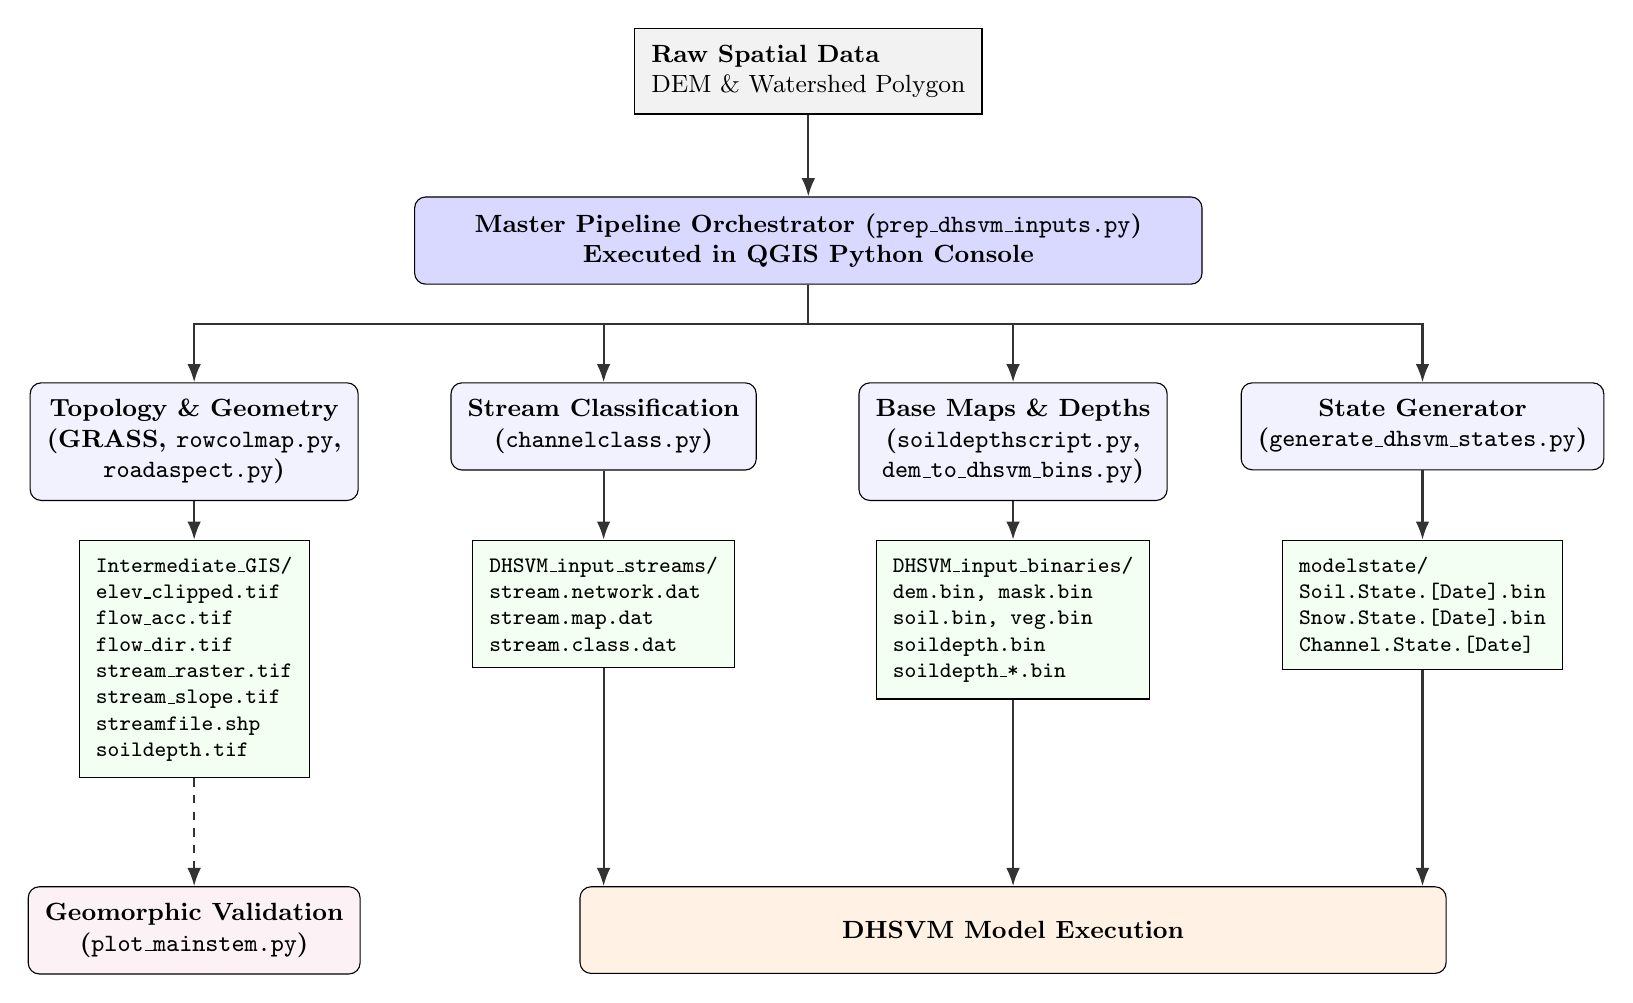
\begin{tikzpicture}[
  >=Latex,
  process/.style={rectangle, rounded corners, draw, align=center, fill=blue!5, font=\small\bfseries, inner sep=6pt, minimum height=1.1cm},
  data/.style={rectangle, draw, align=left, fill=green!5, font=\footnotesize\ttfamily, inner sep=6pt},
  validation/.style={rectangle, rounded corners, draw, align=center, fill=purple!5, font=\small\bfseries, inner sep=6pt, minimum height=1.1cm},
  arrow/.style={->, thick, draw=black!80}
]

% ---------------------------------------------------
% Coordinate Grid (Enforces Perfect Alignment)
% ---------------------------------------------------
\def\xGrass{-7.8}
\def\xStreams{-2.6}
\def\xBins{2.6}
\def\xStates{7.8}

\def\yMaster{0}
\def\yInputs{1.6}
\def\yLayerThree{-1.8}
\def\yLayerFour{-3.8}
\def\yLayerFive{-8.2}

% ---------------------------------------------------
% 1. Inputs & Master (Centered at X=0)
% ---------------------------------------------------
\node[process, fill=blue!15, minimum width=10cm] (master) at (0, \yMaster) {Master Pipeline Orchestrator (\texttt{prep\_dhsvm\_inputs.py})\\Executed in QGIS Python Console};

\node[data, fill=gray!10, font=\small, anchor=south] (inputs) at (0, \yInputs) {\textbf{Raw Spatial Data}\\DEM \& Watershed Polygon};

% ---------------------------------------------------
% 2. Sub-modules (Top edge aligned via anchor=north)
% ---------------------------------------------------
\node[process, anchor=north] (grass) at (\xGrass, \yLayerThree) {Topology \& Geometry\\(GRASS, \texttt{rowcolmap.py},\\ \texttt{roadaspect.py})};

\node[process, anchor=north] (streams) at (\xStreams, \yLayerThree) {Stream Classification\\(\texttt{channelclass.py})};

\node[process, anchor=north] (bins) at (\xBins, \yLayerThree) {Base Maps \& Depths\\(\texttt{soildepthscript.py},\\ \texttt{dem\_to\_dhsvm\_bins.py})};

\node[process, anchor=north] (states) at (\xStates, \yLayerThree) {State Generator\\(\texttt{generate\_dhsvm\_states.py})};

% ---------------------------------------------------
% 3. Output Directories (Top edge aligned)
% ---------------------------------------------------
\node[data, anchor=north] (out_inter) at (\xGrass, \yLayerFour) {\textbf{Intermediate\_GIS/}\\elev\_clipped.tif\\flow\_acc.tif\\flow\_dir.tif\\stream\_raster.tif\\stream\_slope.tif\\streamfile.shp\\soildepth.tif};

\node[data, anchor=north] (out_stream) at (\xStreams, \yLayerFour) {\textbf{DHSVM\_input\_streams/}\\stream.network.dat\\stream.map.dat\\stream.class.dat};

\node[data, anchor=north] (out_bin) at (\xBins, \yLayerFour) {\textbf{DHSVM\_input\_binaries/}\\dem.bin, mask.bin\\soil.bin, veg.bin\\soildepth.bin\\soildepth\_*.bin};

\node[data, anchor=north] (out_state) at (\xStates, \yLayerFour) {\textbf{modelstate/}\\Soil.State.[Date].bin\\Snow.State.[Date].bin\\Channel.State.[Date]};

% ---------------------------------------------------
% 4. Execution & Validation (Top edge aligned)
% ---------------------------------------------------
\node[process, fill=orange!10, minimum width=11cm, anchor=north] (dhsvm) at (\xBins, \yLayerFive) {DHSVM Model Execution};

\node[validation, anchor=north] (valid) at (\xGrass, \yLayerFive) {Geomorphic Validation\\(\texttt{plot\_mainstem.py})};

% ---------------------------------------------------
% Draw Connections
% ---------------------------------------------------
\draw[arrow] (inputs) -- (master);

\draw[arrow] (master.south) -- ++(0,-0.5) -| (grass.north);
\draw[arrow] (master.south) -- ++(0,-0.5) -| (streams.north);
\draw[arrow] (master.south) -- ++(0,-0.5) -| (bins.north);
\draw[arrow] (master.south) -- ++(0,-0.5) -| (states.north);

\draw[arrow] (grass) -- (out_inter);
\draw[arrow] (streams) -- (out_stream);
\draw[arrow] (bins) -- (out_bin);
\draw[arrow] (states) -- (out_state);

\draw[arrow, dashed] (out_inter) -- (valid);

\draw[arrow] (out_stream) -- (out_stream |- dhsvm.north);
\draw[arrow] (out_bin) -- (out_bin |- dhsvm.north);
\draw[arrow] (out_state) -- (out_state |- dhsvm.north);

\end{tikzpicture}%
}
\caption{Architecture of the pure Python DHSVM spatial preparation workflow. Solid arrows indicate the production pipeline; the dashed arrow indicates the optional geomorphic QA branch driven by \texttt{plot\_mainstem.py}.}
\label{fig:workflow}
\end{figure}

%=================================================================
% Appendices
%=================================================================
\newpage
\appendix
\section{Full QGIS Console Execution Log}
\label{app:console_log}

The following log demonstrates the successful execution of the single-step master pipeline (\texttt{prep\_dhsvm\_inputs.py}) for the AR watershed, outputting directly to the strict directory architecture.

\begin{lstlisting}[style=bashstyle,caption={Full console log of the DHSVM spatial pipeline execution.}]
# Python Console
# Use iface to access QGIS API interface or type '?' for more info
# Security warning: typing commands from an untrusted source can harm your computer
exec(compile(Path('/Users/benthosyy/Desktop/CreateStreamNetwork_PythonV/DEM_AR_0406/scripts/prep_dhsvm_inputs.py').read_text(), '/Users/benthosyy/Desktop/CreateStreamNetwork_PythonV/DEM_AR_0406/scripts/prep_dhsvm_inputs.py', 'exec'))

=======================================================
  DHSVM SPATIAL PIPELINE INITIALIZING
=======================================================
[ok] Watershed polygon: arwd_watershed_UTM17.shp
[ok] Master DEM: elev_clipped.tif
[info] Cell area (*@$\approx$@*) 792.858 m(*@$^2$@*)
[info] MIN_SRC_AREA (m(*@$^2$@*)) = 47571.500  (from 60 cells)
[step] Clipping DEM to watershed...
[ok] Working DEM ready: elev_clipped.tif
[step] GRASS r.watershed -> flow direction & accumulation...
[step] GRASS r.stream.extract -> extracting streams...
[step] GRASS r.slope.aspect -> calculating slope...
[step] Routing classifications to DHSVM_input_streams/...
stream.class.dat written: /Users/benthosyy/Desktop/CreateStreamNetwork_PythonV/DEM_AR_0406/DHSVM_input_streams/stream.class.dat
Class counts: {13: 30}
[info] Slope mode auto-detected as: tan (converted to tan for binning)
[step] Writing topologic stream files to DHSVM_input_streams/...
[step] Compute Soil Depth Binary (soildepthscript.py)...
  [soildepth] Reading spatial inputs into memory...
  [soildepth] Aligning boundaries and sanitizing edge pixels...
  [soildepth] Computing weighted topograpic functions...
  [soildepth] Writing flat binary -> soildepth.bin
  [soildepth] Writing GeoTIFF -> soildepth.tif
  [soildepth] Complete.
[step] Generate DHSVM Base Maps (dem_to_dhsvm_bins.py)...

--- Initializing DHSVM Base Map Generation Pipeline ---
[step] Reading master topography: elev_clipped.tif
[step] Structuring physical memory arrays (Float32 and Int8)...
[step] Serializing standard base maps to: DHSVM_input_binaries/
  -> Generated: dem.bin  (Float32)
  -> Generated: mask.bin (Int8)
  -> Generated: soil.bin (Int8)
  -> Generated: veg.bin  (Int8)

[step] Generating uniform soil depth baselines...
  -> Generated: soildepth_uniform_2.0m.bin (Float32)
  -> Generated: soildepth_uniform_2.5m.bin (Float32)
  -> Generated: soildepth_uniform_3.0m.bin (Float32)
  -> Generated: soildepth_uniform_3.5m.bin (Float32)
  -> Generated: soildepth_uniform_4.0m.bin (Float32)

[SUCCESS] DHSVM spatial base maps and depth baselines successfully generated!
[step] Generate DHSVM Initial States (generate_dhsvm_states.py)...

=======================================================
  DHSVM PURE PYTHON STATE INITIALIZER
=======================================================

[step] Generating binary grid states for 01.01.2016.00.00.00 (NY=55, NX=72)
  -> Interception.State.01.01.2016.00.00.00.bin (pure Python binary)
  -> Snow.State.01.01.2016.00.00.00.bin (pure Python binary)
  -> Soil.State.01.01.2016.00.00.00.bin (pure Python binary)
[step] Generating physics-based channel states -> Channel.State.01.01.2016.00.00.00
=======================================================


=======================================================
  PIPELINE FINISHED SUCCESSFULLY
=======================================================
STREAM FILES:  DHSVM_input_streams/
BINARY GRIDS:  DHSVM_input_binaries/
MODEL STATES:  modelstate/
INTERMEDIATE:  Intermediate_GIS/
\end{lstlisting}

\end{document}
